% File: jupiter-css-podc16-c1234-css1.tex

\documentclass{standalone}

% preamble for jupiter-paper related TikZ drawing
\usepackage{tikz}
\usetikzlibrary{shapes, positioning, arrows.meta, calc, backgrounds, fit}

% default horizontal/vertical distance
\def\hdist{1.8}
\def\vdist{1.8}

\newcommand{\state}[2]{% #1: state label; #2: position
  \node (#1) [circle, inner sep = 0pt, minimum size = 10mm, text width = 10mm, align = center, draw, #2, font = \Large] {$#1$};
}

\tikzset{every lower node part/.style = {red}}
\newcommand{\statesplit}[3]{% #1: state upper label; #2: state lower label; #3: position
  \node (#1) [circle split, draw, minimum size = 6mm, text width = 10mm, align = center, #3, font = \Large]
  {
	$#1$
	\nodepart{lower}
	$#2$
  };
}

\newcommand{\transition}[4][]{% #2: start state; #3: end state; #4: transition label; #1: transition label position (optional)
  \draw[>=Stealth, ->] (#2) to node [rectangle, draw, above = 2pt, sloped, #1, font = \small] {#4} (#3);
}

\newcommand{\ins}[2]{$\textsc{Ins}(#1,#2)$}
\newcommand{\del}[2]{$\textsc{Del}(#1,#2)$}

\tikzset{node distance = \vdist and \hdist}
\tikzset{path/.style = {draw, rounded corners, very thick, #1}}

\begin{document}
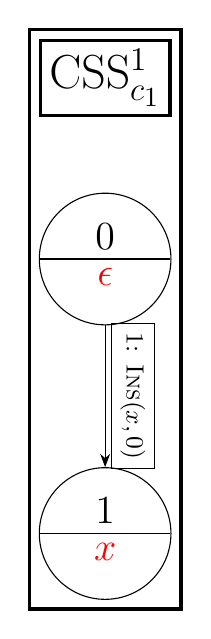
\begin{tikzpicture}[css/.style = {font = \LARGE, rectangle, draw, very thick},
	bg/.style = {rectangle, draw, very thick}]
  \statesplit{0}{\epsilon}{}
  \statesplit{1}{x}{below = of 0}
  \transition{0}{1}{1: \ins{x}{0}}

  \begin{pgfonlayer}{background}
    \node (ss) [css, above = of 0.center] {CSS$_{c_1}^{1}$};
    \node () [fit = (0) (1) (ss), bg] {};
  \end{pgfonlayer}
\end{tikzpicture}
\end{document}
